\documentclass[a4paper,
fontsize=11pt,
%headings=small,
oneside,
numbers=noperiodatend,
parskip=half-,
bibliography=totoc,
final
]{scrartcl}

\usepackage[babel]{csquotes}
\usepackage{synttree}
\usepackage{graphicx}
\setkeys{Gin}{width=.4\textwidth} %default pics size

\graphicspath{{./plots/}}
\usepackage[ngerman]{babel}
\usepackage[T1]{fontenc}
%\usepackage{amsmath}
\usepackage[utf8x]{inputenc}
\usepackage [hyphens]{url}
\usepackage{booktabs} 
\usepackage[left=2.4cm,right=2.4cm,top=2.3cm,bottom=2cm,includeheadfoot]{geometry}
\usepackage{eurosym}
\usepackage{multirow}
\usepackage[ngerman]{varioref}
\setcapindent{1em}
\renewcommand{\labelitemi}{--}
\usepackage{paralist}
\usepackage{pdfpages}
\usepackage{lscape}
\usepackage{float}
\usepackage{acronym}
\usepackage{eurosym}
\usepackage{longtable,lscape}
\usepackage{mathpazo}
\usepackage[normalem]{ulem} %emphasize weiterhin kursiv
\usepackage[flushmargin,ragged]{footmisc} % left align footnote
\usepackage{ccicons} 
\setcapindent{0pt} % no indentation in captions

%%%% fancy LIBREAS URL color 
\usepackage{xcolor}
\definecolor{libreas}{RGB}{112,0,0}

\usepackage{listings}

\urlstyle{same}  % don't use monospace font for urls

\usepackage[fleqn]{amsmath}

%adjust fontsize for part

\usepackage{sectsty}
\partfont{\large}

%Das BibTeX-Zeichen mit \BibTeX setzen:
\def\symbol#1{\char #1\relax}
\def\bsl{{\tt\symbol{'134}}}
\def\BibTeX{{\rm B\kern-.05em{\sc i\kern-.025em b}\kern-.08em
    T\kern-.1667em\lower.7ex\hbox{E}\kern-.125emX}}

\usepackage{fancyhdr}
\fancyhf{}
\pagestyle{fancyplain}
\fancyhead[R]{\thepage}

% make sure bookmarks are created eventough sections are not numbered!
% uncommend if sections are numbered (bookmarks created by default)
\makeatletter
\renewcommand\@seccntformat[1]{}
\makeatother

% typo setup
\clubpenalty = 10000
\widowpenalty = 10000
\displaywidowpenalty = 10000

\usepackage{hyperxmp}
\usepackage[colorlinks, linkcolor=black,citecolor=black, urlcolor=libreas,
breaklinks= true,bookmarks=true,bookmarksopen=true]{hyperref}
\usepackage{breakurl}

%meta
%meta

\fancyhead[L]{S. Sparber\\ %author
LIBREAS. Library Ideas, 40 (2021). % journal, issue, volume.
\href{https://doi.org/10.18452/23803}{\color{black}https://doi.org/10.18452/23803}
{}} % urn 
% recommended use
%\href{http://nbn-resolving.de/}{\color{black}{urn:nbn:de...}}
\fancyhead[R]{\thepage} %page number
\fancyfoot[L] {\ccLogo \ccAttribution\ \href{https://creativecommons.org/licenses/by/4.0/}{\color{black}Creative Commons BY 4.0}}  %licence
\fancyfoot[R] {ISSN: 1860-7950}

\title{\LARGE{kolonial geordnet: die historische Bestandsanalyse als Methode zum Aufspüren von Othering in Bibliotheksbeständen
}}% title
\author{Sandra Sparber} % author

\setcounter{page}{1}

\hypersetup{%
      pdftitle={kolonial geordnet: die historische Bestandsanalyse als Methode zum Aufspüren von Othering in Bibliotheksbeständen
},
      pdfauthor={Sandra Sparber},
      pdfcopyright={CC BY 4.0 International},
      pdfsubject={LIBREAS. Library Ideas, 40 (2021).},
      pdfkeywords={Bibliothek, Dekolonisierung, library, decolonization},
      pdflicenseurl={https://creativecommons.org/licenses/by/4.0/},
      pdfcontacturl={http://libreas.eu},
      baseurl={https://doi.org/10.18452/23803},
      pdflang={de},
      pdfmetalang={de}
     }



\date{}
\begin{document}

\maketitle
\thispagestyle{fancyplain} 

%abstracts

%body
\hypertarget{einleitung}{%
\section{Einleitung}\label{einleitung}}

Vor mehr als zehn Jahren katalogisierte ich die Missio-Sondersammlung,
eine etwa 6.500 Werke umfassende Dauerleihgabe, die von \emph{MISSIO
Österreich}\footnote{Die verschiedenen Schreibweisen von Missio sind den
  Eigenbezeichnungen der diversen Einrichtungen geschuldet. Diese werden
  im vorliegenden Text beibehalten und stellen sich folgendermaßen dar:
  MISSIO Österreich und missio Aachen. Der untersuchte Teilbestand der
  einstigen Missio-Bibliothek wird als Missio-Sondersammlung oder
  Missio-Bestand bezeichnet.} -- dem österreichischen Zweig der
Päpstlichen Missionswerke -- an die \emph{Bibliothek der
Österreichischen Forschungsstiftung für Internationale Entwicklung
(ÖFSE)} gegangen war. Es stellte sich schnell heraus, dass der Bestand
von rassistischen Inhalten durchzogen war. 2019, ich hatte noch Kontakt
zu einigen Kolleg:innen,\footnote{Im Text wird geschlechtersensible
  Schreibweise praktiziert, indem mittels Doppelpunkt Personen jenseits
  der binären Zuschreibung von Mann/Frau berücksichtigt werden sollen.
  Dort, wo der inhaltliche oder historische Kontext nicht darauf
  schließen lässt, dass Personen oder Gruppen Geschlechteridentitäten in
  Frage stellen oder gestellt haben, werden sie innerhalb des binären
  Systems verortet.} ergab sich die Möglichkeit, mich näher mit diesem
Bestand, der mittlerweile der Bibliothek geschenkt worden war,
auseinanderzusetzen. Zwischenzeitlich hatten sich Studierende über
rassistische Werke in diesem Teilbestand beschwert. Mein Ziel war es,
exemplarisch an dieser Sammlung eine Methode zu entwickeln, die dazu
beitragen sollte, koloniale Repräsentationen in Beständen aufzuspüren,
ohne dabei jedes einzelne Buch analysieren zu müssen. Es sollte sich um
eine im ressourcenknappen Bibliotheksalltag praxistaugliche
Anwendungsmöglichkeit handeln.

Ausgangspunkt dieser historischen Bestandsanalyse ist die Annahme, dass
sich koloniale Repräsentationen auf drei Ebenen in die Sammlung
eingeschrieben haben, nämlich dass wir sie in der Disziplin selbst,
innerhalb der verwendeten Wissensordnung und auf Ebene der Texte finden.
Rassistische Denkmuster, die an verschiedenen Stellen der
Missionswissenschaft (re)pro\-duziert werden, würden sich demnach als
sozial konstruierte Auf- und Abwertungen in Form von Othering\footnote{\enquote{Von
  Othering spricht man, wenn eine Gruppe oder eine Person sich von einer
  anderen Gruppe abgrenzt, indem sie die nicht-eigene Gruppe als
  andersartig und fremd beschreibt. Dies geschieht in der Regel
  innerhalb eines Machtgefälles: die als anders Beschriebenen sind von
  Diskriminierung betroffen und haben deswegen wenig Möglichkeiten, sich
  gegen die Zuschreibung zu wehren.}
  (\url{https://diversity-arts-culture.berlin/woerterbuch/othering})} in den
entsprechenden Gruppen der internen Klassifikation finden. Dort wiederum
wäre eine Häufung an rassistischen Büchern auszumachen, so meine
Vermutung.

Um dies zu überprüfen wird der Missio-Bestand und sein Sammelgebiet
historisch und wissenschaftsgeschichtlich zu kontextualisieren sein.
Danach erfolgt die Analyse der Klassifikation. Um abschließend
feststellen zu können, ob sich in den als problematisch beschriebenen
Gruppen tatsächlich mehr rassistische Titel finden als in anderen,
werden Stichproben aus dem Gesamtbestand gezogen und die Werke
inhaltsanalytisch auf Rassismen untersucht. Das vorgestellte Instrument
ist ausschließlich auf einen abgeschlossenen, klassifikatorisch
geordneten Bestand abgestimmt.

\hypertarget{ordnung-und-wissen}{%
\section{Ordnung und Wissen}\label{ordnung-und-wissen}}

Theoretisch fußt meine Herangehensweise auf den Prämissen von Michel
Foucault, wonach Wissen im Kontext von Machtgefügen entsteht und als
konstruierte Bedeutung gesellschaftlich anerkannte Wahrheit
generiert.\footnote{Vergleiche Foucault (1981), S. 259} Wissen ist
demnach keine Aussage über eine objektive Wahrheit, sondern erkämpfte
Bedeutung. Der Austragungsort um diese Deutungshoheit ist der Diskurs.
Er ist \emph{\enquote{dasjenige, worum und womit man kämpft; er ist die
Macht, derer man sich zu bemächtigen versucht.}}\footnote{Derselbe
  (2012), S. 11} Machtkonstellationen, die sich institutionalisieren und
innerhalb eines Diskurses als strategische und reproduktive Mechanismen
in Erscheinung treten, bezeichnet Foucault als Dispositive.\footnote{Vergleiche
  ders. (1983), S. 62} Explizit führt er Bibliotheken als Dispositiv an,
aufgrund der \emph{\enquote{Art und Weise, wie {[}\ldots{]} Wissen in
einer Gesellschaft eingesetzt {[}\ldots{]}, gewertet und sortiert,
verteilt und zugewiesen wird.}}\footnote{Derselbe (2012), S. 15}

In \emph{Die Ordnung der Dinge} geht Foucault der Frage nach der
Entstehung von wissenschaftlichem Wissen nach und stellt fest, dass es
im 17. Jahrhundert zu einer Verschiebung kommt, weg von den
Ähnlichkeiten als maßgebendes Wesensmerkmal ordnender Elemente hin zu
den Unterschieden.\footnote{Vergleiche ders. (2019), S. 83\,ff.} Es
folgen Wissensordnungen wie etwa Carl von Linnés \emph{systemae naturae}
von 1758, wo Identität und Unterschied mit sozialen Auf- und Abwertungen
verknüpft werden. Linnés Ordnungssystem zementiert das Bild des
fleißigen Europäers und des trägen Afrikaners.\footnote{Vergleiche
  Schrenk, 2018, S. 46} Stark vereinfacht entspricht dieser Prozess der
Abwertung jenem Phänomen, das Gayatri Chakravorty Spivak als Othering
bezeichnet.\footnote{Vergleiche Spivak (1985)}

Wenn nun also eine Gruppe von Menschen mittels Othering, sei es aufgrund
von Geschlecht, Klasse, ethnischer Zugehörigkeit, Religion, sexueller
Präferenz, Nation oder anderen Unterscheidungsmerkmalen, zum
vermeintlich unterlegenen Fremden und das vermeintlich überlegene Eigene
zum selbstreferentiellen Bezugspunkt wird, führt dies zu sozial
konstruierten Ungleichverhältnissen. Folglich können sich diese als
Differenzen manifestieren, welche diskursiv reproduziert werden. Das
Abbilden in Wissensordnungen ist gleichsam Konsequenz und Ausgangslage
von Wissensgenerierung. Durch ihre Anwendung reproduzieren wir eine
Geisteshaltung.\footnote{Hope Olson hat etwa die Privilegierung
  westlicher Kulturen in den Sprachgruppen der
  Dewey-Dezimalklassifikation nachgewiesen. Weitere Informationen:
  Vergleiche Olson, 2001, S. 115\,ff.} Diese müsste sich eingeschrieben
haben in:

a) die verschiedene Bereiche der Disziplin bzw. des Sammelgebiets

b) die Klassifikation und

c) die Werke

Nach einer kurzen Beschreibung der ethnozentrischen Dimensionen des
Sammelgebiets wird die Analyse auf Ebene der Klassifikation und der
Werke erfolgen, um Reproduktionen kolonialer Geisteshaltungen
aufzuspüren.

\hypertarget{die-missio-sammlung}{%
\section{Die Missio-Sammlung}\label{die-missio-sammlung}}

Die Gründungsgeschichte der Sammlung lässt sich nicht im Detail
nachzeichnen, obwohl Gespräche mit Mitarbeiterinnen von \emph{MISSIO}
geführt wurden. Es kann aber angenommen werden, dass frühe Bestände
lange Zeit als Handbibliothek der Päpstlichen Missionswerke dienten und
zum Schutz vor der Zerschlagung durch die Nationalsozialisten 1938 dem
Missiologischen Institut zugeführt wurden.\footnote{So wurde 1938 die
  missionswissenschaftliche Lehrtätigkeit an der Universität Wien
  untersagt. Als Folge gründete der Wiener Kardinal Theodor Innitzer
  zwei Missionsabteilungen in der Erzdiözese Wien, die Abteilung
  Missionswesen für Propagandatätigkeiten und das Missiologische
  Institut für die wissenschaftliche Forschung. Siehe: Bettray (1954),
  S. 57\,f.} Stempelvermerke deuten auch auf zahlreiche Schenkungen
anderer Einrichtungen wie etwa der Marianischen Frauen- und
Jungfrauen-Congregation oder dem Katechetischen Museum Wien hin. Als
sich die Päpstlichen Missionswerke in Österreich in den 1990er Jahren in
\emph{MISSIO} umbenannten, konnten sie auf eine bereits 150-Jährige,
äußerst erfolgreiche Geschichte zurückblicken. Institutionell versteht
sich \emph{MISSIO} als Nachfolgeorganisation des 1822 gegründeten Lyoner
Missionsvereins. 1922 erfolgte die innerkirchliche Zentralisierung durch
die Eingliederung in die Päpstlichen Missionswerke, die der Kongregation
der Evangelisierung der Völker unterstellt sind.\footnote{Vergleiche.
  Kainberger (2014), S. 7} In den 1820er Jahren verzeichneten einzelne
Missionsvereine bereits bis zu 100.000 Mitglieder.\footnote{Vergleiche
  Faschingeder (2002), S. 11} Zu Beginn des 20. Jahrhunderts waren sie
oft zu enormen Unternehmen mit eigenen Druckereien, Verlagen und
Bildungseinrichtungen angewachsen. Ihr Ziel war und blieb die
finanzielle Unterstützung der verschiedenen Missionen. 2018 zählte der
nationale Ableger von \emph{MISSIO} mit einem Spendenaufkommen von etwa
zehn Millionen Euro zu einer der größten Fundraising-Organisationen in
Österreich.\footnote{Vergleiche Fundraising Verband Austria (2019), S.
  22
  (\url{http://public-opinion.at/wp-content/uploads/2019/11/Spendenbericht_2019_v10-WEB.pdf}
  überprüft am 18.05.2021)} Die Bibliothek erfuhr in den 1980er Jahren
eine Professionalisierung. Bestände wurden zusammengeführt,
katalogisiert und anhand einer eigenen Klassifikation inhaltlich
geordnet. Der Medienzuwachs erfolgte über Schenkungen, Nachlässe und
projektbezogenen Ankauf. Bis in die 1990er Jahre galt die gesamte
Einrichtung kirchenintern als linker Flügel, da in den Jahrzehnten zuvor
befreiungstheologischen Inhalten eine hohe Bedeutung zugekommen war.
2008 wurde die \emph{MISSIO}-Bibliothek aufgelassen.\footnote{Die
  Informationen zur Geschichte der Bibliothek ab den 1980er Jahren
  stammen aus einem Gespräch der Autorin mit zwei
  Missio-Mitarbeiterinnen, das 2019 geführt wurde.} Neben jenen Medien,
die 2009 an die \emph{ÖFSE} gegangen waren, wurde ein weiterer
Teilbestand der \emph{Missionsbibliothek und katholischen
Dokumentationsstelle} von \emph{missio Aachen} (MIKDAO) übergeben;
darunter eine Sammlung sehr seltener Katechismen in außereuropäischen
Sprachen.\footnote{Vergleiche Richter (2019), S. 9\,ff}

Im kolonialen Wissen, also in den gesellschaftlich anerkannten
Wahrheiten, deren Bedeutungen im Kontext der europäischen Expansion
generiert wurden, war die Annahme einer weißen Überlegenheit bereits
angelegt. Lokale Gesellschaftsformen wurden als unterentwickelt
bezeichnet. Fremde spirituelle Überzeugungen erfuhren als Aberglauben
eine Abwertung in Abgrenzung zum eigenen Glauben, der christlichen
Religion.\footnote{Vergleiche Habermas (2010), S. 258\,f.}
Systematisierungsansprüche führten dazu, dass zahlreiche Laien und
Amateurforscher durch das Erfassen, Vermessen, Ein- und Zuordnen von
Gebieten, Fauna, Flora und Menschen verwissenschaftlichtes Wissen
schufen.\footnote{Vergleiche ebenda} Am regen Informationsaustausch
zwischen den Kolonien und ihren Mutterländern waren neben
Kolonialbeamten, Forschenden, Reisenden und Siedlern auch Missionare
beteiligt. In Berichten, Vorträgen und Zeitschriftenartikeln
vermittelten sie nicht nur Wissen, das für die Ausbeutung der Gebiete
von Bedeutung war, wie etwa Hinweise zu Rohstoffvorkommen,
Witterungsbedingungen et cetera. Sie transportierten dabei auch
imaginierte Vorstellungen von Gesellschaft, Kultur und Natur der
unterworfenen Länder. Missionszeitschriften und -ausstellungen trugen
das ihrige dazu bei. Umgekehrt produzierten Missionsverlage hohe
Auflagen an gedruckten Werken für die Missionen wie etwa Katechismen
oder Gebetsbücher.\footnote{Vergleiche Bettray (1954), S. 40} Mit der
Glaubenserziehung einher gingen meist auch soziale und kulturelle
Disziplinierungsansprüche wie das Annehmen von Bekleidungstraditionen,
Sprach-, Rechts- und Körperpraktiken aber auch von bestimmten
Arbeitsweisen.\footnote{Vergleiche Faschingeder (2002), S. 7} Nicht
selten übernahmen Missionare koloniale Aufgaben, wenn sie sich etwa als
Kartografen betätigten, Schätzungen zur Größe lokaler
Bevölkerungsgruppen abgaben oder sich als Dolmetsch zur Verfügung
stellten.\footnote{So unterzeichnete der Rheinische Missionar Johannes
  Heinrich Bam als Zeuge 1883 den betrügerischen Vertrag des
  Landverkaufs der Nama durch Josef David Frederiks und dem
  Kolonialpionier Adolf Lüderitz sowie im darauffolgenden Jahr als
  Dolmetsch den Schutzvertrag zwischen dem Deutschen Reich und dem
  Einflussgebiet Josef Frederiks. Somit war ein Missionar direkt an der
  Errichtung der Siedlungskolonie im heutigen Namibia beteiligt.
  Weiterführende Informationen siehe: Drechsler: Südwestafrika unter
  deutscher Kolonialherrschaft, 1984.}

Die Herausforderung, einen missionswissenschaftlichen Bestand in
Hinblick auf Othering zu untersuchen, besteht darin, nicht den
inhaltlichen Sammelschwerpunkt als Ganzes den Praktiken der
\emph{VerAnderung} zuzuordnen. Dies ist insofern schwierig als der
Ausgangspunkt von Missionierung ebenfalls das Eigene dem Fremden
gegenüberstellt und die kirchliche Lehre eine Abwertung von Ungläubigen
(bis hin zu Verfolgungs- und Vernichtungspolitiken) kennt. Diesen Aspekt
versuche ich zu entschärfen, indem ich bei der Analyse dem
missionierenden Subjekt in bester Absicht unterstelle, sein Gegenüber
als autonomes und gleichwertiges Wesen zu begreifen. Religionsimmanente
Zuschreibungen bleiben unberücksichtigt, während explizite
Selbsterhöhung und/oder Fremdabwertung in den unterschiedlichen Facetten
als Othering begriffen wird.

\hypertarget{die-missio-klassifikation}{%
\section{Die
Missio-Klassifikation}\label{die-missio-klassifikation}}

Der Missio-Bestand folgt einer klassifikatorischen Ordnung, bestehend
aus 19 Hauptgruppen mit bis zu elf Untergruppen. Neun Hauptgruppen
werden in den Notationen mit Lateinischen Buchstaben (allgemeine
bestandsspezifische Wissensgebiete), zehn Hauptgruppen mit Römischen
Ziffern (geografische Zuordnungen) dargestellt, gefolgt von
fortlaufenden Nummern, welche den Stellplatz des einzelnen Exemplars im
Regal beschreiben. Entworfen wurde die Klassifikation von \emph{MISSIO}.
Sie wurde von der ÖFSE unverändert übernommen und ist für Leser:innen
frei zugänglich an den Regalen angebracht.

\begin{figure}
\centering
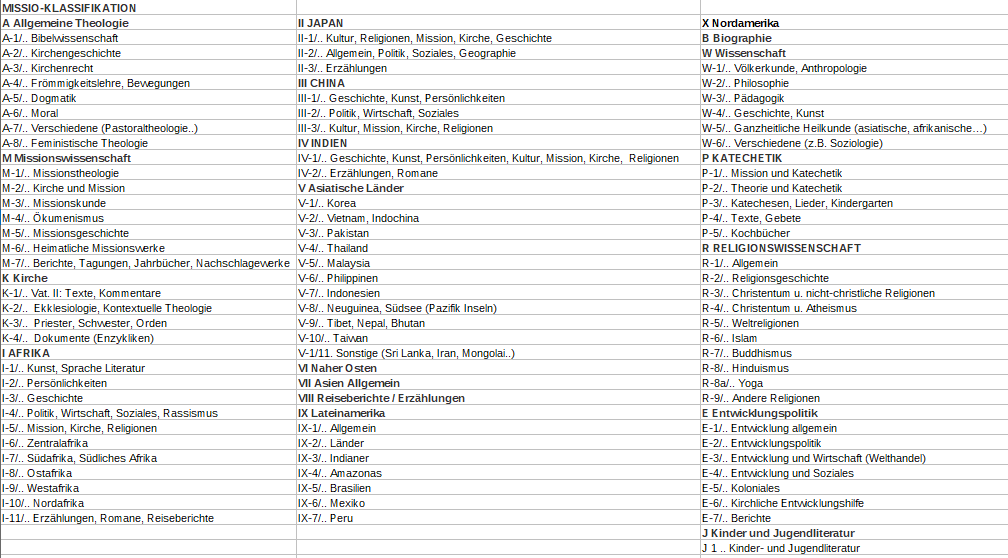
\includegraphics[width=.99\textwidth]{img/img1.PNG}
\caption{MISSIO-Klassifikation (Sparber, 2019)}
\end{figure}

Sieht man von formalen Inkonsequenzen wie etwa der Unterbrechung in der
Abfolge von allgemeinen Wissensgebieten (Buchstaben) durch geografische
Einheiten (Römische Zahlen) oder der Wiederholung der Bezeichnung von
Hauptgruppen in ihren Untergruppen ab, lassen sich an folgenden Stellen
in der Klassifikation Dimensionen von Othering nachweisen:

\begin{itemize}
\item
  Im Bereich der geografischen Hauptgruppen (I--X) kann das Fehlen der
  Kategorie Europa als Normierung des Eigenen gelesen werden. Obwohl
  innereuropäische Missionierung historisch belegt ist, bleibt Europa
  ungenannter selbstreferentieller Bezugspunkt und die Abweichung davon
  konstruiert das Andere, das es zu benennen gilt.
\item
  Innerhalb der geografischen Hauptgruppen erfolgt eine Hierarchisierung
  der verschiedenen Gebiete und ihrer Benennung, wenn etwa Kontinente
  (\emph{Afrika}), Länder (zum Beispiel \emph{Japan}, \emph{China}) und
  regionale Bezeichnungen (\emph{Naher Osten}) auf gleicher Ebene
  genannt werden. Dies impliziert eine Abwertung kultureller und
  sozialer Errungenschaften der großen geografischen Einheiten. Ihre
  Leistungen auf den verschiedenen Gebieten benötigen nicht mehr
  inhaltliche Breite und Tiefe als jene mancher Länder, die ebenfalls in
  den Hauptgruppen geführt werden. Dieser Umstand deckt sich auch mit
  den Stichproben, wo insbesondere die sogenannten Hochkulturen Japans,
  Chinas und Indiens (allesamt als Hauptgruppen geführt), entsprechende
  Anerkennung in den Publikationen europäischer Autoren finden und somit
  eine weniger starke Abwertung im Vergleich zu afrikanischen Kulturen
  erfahren (was wiederum nicht bedeutet, dass dort keine rassistischen
  Inhalte zu finden sind). Die Gleichsetzung des Kontinents Afrika mit
  den genannten Ländern führt zur Konstruktion einer kulturellen und
  sozialen afrikanischen Gesamtheit und kollektiven Unterlegenheit.
  Regionale Diversität wird komplett ausgeblendet während sie bei den in
  den Hauptgruppen geführten Ländern nennenswert erscheint.
\item
  Eine weitere Auffälligkeit auf Ebene der Hauptgruppen bildet die
  Hauptgruppe \emph{Asien Allgemein}; kein anderer Kontinent verfügt
  über diese oder überhaupt eine zusätzliche Hauptgruppe. Asien ist in
  der Klassifikation mit sechs Nennungen auf erster Ebene
  überrepräsentiert.
\item
  Unter den geografischen Hauptgruppen enthalten nur der \emph{Nahe
  Osten}, \emph{Asien Allgemein} und \emph{Nordamerika} keine
  Untergruppen. Ausgeblendet wird somit der Umstand, dass es
  missionierende Kirchen etwa in den USA gibt, die ihr Hauptaugenmerk
  eventuell nicht auf die indigene Bevölkerung richten. Eventuell ist
  die Nicht-Nennung nicht nur Folge des üblicherweise ungenannten
  Eigenen, sondern auch auf eine geringe Medienanzahl innerhalb dieser
  Abteilung zurückzuführen. Der Mangel einer systematischen Anordnung
  von Vergleichbarem auf gleicher Ebene setzt sich auch in den
  Untergruppen fort. An dieser Stelle kann auch die Frage nach dem Grund
  nicht vorhandener Medien und somit nicht vorhandener Gruppen
  aufgeworfen werden. Eventuell wurde dem Thema bislang keine
  publizistische Aufmerksamkeit geschenkt. Oder aber, es handelt sich um
  einen blinden Fleck im Bestandsaufbau. Da der Buchankauf in der
  Missio-Bibliothek projektbezogen erfolgte, ist es naheliegend, dass
  solche Auslassungen den organisationsspezifischen Schwerpunkten
  zugrunde liegen.
\item
  Auch im Bereich der Untergruppen lassen sich Zuschreibungen ausmachen,
  die als Ausdruck von Othering verstanden werden können. So weist die
  Untergruppe 4 der Hauptgruppe \emph{Afrika} die Entitäten
  \emph{Politik}, \emph{Wirtschaft}, \emph{Soziales} und
  \emph{Rassismus} auf. Im Wissen, dass die Klassifikation in den 1980er
  Jahren angelegt worden ist, zu einem Zeitpunkt als ein Großteil der
  afrikanischen Länder formal ihre politische Unabhängigkeit bereits
  erlangt hatte, ist die Aneinanderreihung von Kategorien, die
  weitgehend im Bereich der afrikanischen Staaten selbst liegen,
  schlüssig. Diese allerdings mit \emph{Rassismus} abzuschließen legt
  nahe, dass es sich bei ihm ebenso um ein afrikanisches Phänomen
  handelt. Möchte man den europäischen Rassismus gegenüber afrikanischen
  Personen und gesamten Bevölkerungen abbilden, wäre er als Begriff
  einer europäischen Kategorie zuzuordnen. Wollte man die
  gesamtgesellschaftlichen Auswirkungen des europäischen Rassismus in
  Afrika abbilden, wäre hierfür eine passende Bezeichnung wie etwa
  Ausbeutung, Unterdrückung oder Diskriminierung vorzuziehen. Es geht
  hier nicht um den \uline{einen} korrekten Begriff sondern darum, nicht
  den Eindruck zu vermitteln, Rassismus läge wie ein Schleier über
  seinen Opfern, während jene, die ihn ausüben, unsichtbar bleiben.
\item
  Ein weiteres Indiz europäischer Überlegenheit, das in der
  Klassifikation ihren Ausdruck findet, ist die Untergruppe E-5 mit der
  Bezeichnung \emph{Koloniales}. Dieses Element ist umgeben von den
  Entitäten \emph{Entwicklungspolitik, Welthandel, Entwicklung} und
  \emph{Soziales} sowie \emph{Kirchliche Entwicklungshilfe} und gehört
  mit ihnen zur Hauptgruppe \emph{Entwicklungspolitik}. Abgesehen davon,
  dass sich die Benennung der Hauptgruppe \emph{Entwicklungspolitik} in
  einer Untergruppe wiederholt, erweckt die Nennung des
  \emph{Kolonialen} in der entsprechenden Gruppe den Eindruck als handle
  es sich dabei um einen Bereich der Entwicklungspolitik.
\item
  Die Hauptgruppe \emph{Lateinamerika} beinhaltet wie die der
  \emph{Asiatischen Länder} nur eine unvollständige Auflistung von
  Ländern. Zudem wird der Begriff \emph{Indianer} als koloniale
  Fremdbezeichnung der indigenen Bevölkerung auf zweiter Ebene der
  Klassifikation verwendet.
\item
  Bezüglich der nicht geografischen Abteilungen der Klassifikation kann
  festgehalten werden, dass hier vor allem die
  \emph{Religionswissenschaft} Othering aufweist, indem die ersten vier
  Untergruppen \emph{Allgemein, Religionsgeschichte, Christentum und
  nicht-christliche Religionen sowie Christentum und Atheismus} das
  Christentum aufgrund der Ausdifferenzierung privilegiert. Ein Umstand,
  der angesichts der Positionierung der sammelnden Einrichtung nicht
  überraschend ist.
\end{itemize}

\hypertarget{die-buxfccher-im-missio-bestand}{%
\section{Die Bücher im Missio-Bestand}\label{die-buxfccher-im-missio-bestand}}

Im November 2009 wurden etwa 6.500 Titel\footnote{Innerhalb der ÖFSE
  gibt es mehrere Bestandslisten, die unterschiedliche Zahlen des
  Gesamtbestands beinhalten. Die Differenz von etwa 500 Einträgen dürfte
  sich aus der Unterscheidung von Exemplaren und Titeln ergeben, so dass
  von einer hohen Anzahl an Dubletten ausgegangen werden kann. Für die
  vorliegende Analyse wurden jene Titelsätze mit Signaturen aus dem
  Bibliothekskatalog herangezogen.} der \emph{ÖFSE} als Dauerleihgabe
mit der Auflage übergeben,\footnote{2018 erfolgte die Schenkung eines
  weiteren Teilbestands. Dabei wurden 115 Bücher von \emph{MISSIO Wien}
  der \emph{Missionsbibliothek und katholischen Dokumentationsstelle
  MIKADO} (missio Aachen) übergeben. 51 dieser Bücher wurden von MIKADO
  ausgewertet (der Rest stellte Dubletten dar). Eine kurze Analyse der
  Verfasserin ergab, dass die drei häufigsten Besitznachweise aus dem
  Katechetischen Museum Wien, der Petrus-Claver-Sodalität und der
  Bibliothek der Oblaten der Unbefleckten Jungfrau stammen. Es handelt
  sich in erster Linie um Katechismen, Volksbibeln, Lieder- und
  Predigtbücher, wobei etwa die Hälfte der Titel in nichteuropäischen
  Sprachen gedruckt wurde. Diese können wiederum über Besitzvermerke der
  Petrus-Claver-Sodalität zugeordnet werden und es liegt nahe, dass die
  Bücher in deren Druckereien, zu denen auch jene in Maria Sorg gehörte,
  gedruckt und als Belegexemplar an das Werk der Glaubensverbreitung
  abgeliefert worden waren. Die in der Schenkung enthaltenen Titel
  erschienen im Zeitraum zwischen 1853 und 1991, wobei der größte Teil
  im ersten Drittel des 20. Jahrhunderts publiziert wurde. Weitere
  Informationen siehe Richter: Der Bestand von missio Wien in der
  Missionsbibliothek und katholischen Dokumentationsstelle von missio
  Aachen, 2019.} den Bestand geschlossen aufzustellen; 2018 erfolgte
dann die Schenkung des Bestands.\footnote{E-Mail der Bibliotheksleitung
  an die Verfasserin vom 19.2.2020} Die Untersuchung der Klassifikation
und der Medien erfolgte im Dezember 2019. Das Datenmaterial, dem die
Analyse zugrunde liegt, umfasst die Wissensordnung in Form der
Klassifikation, die den Bestand inhaltlichen Schwerpunkten zuordnet. Sie
dient gleichzeitig als Aufstellungssystematik. Neben dem
Bibliothekskatalog, in dem sämtliche Exemplare des Missio-Bestands
verzeichnet sind, erhielt die Verfasserin von einem
Bibliotheksmitarbeiter eine Excel-Datei mit sämtlichen Titeln aus der
Sondersammlung. Die Stichproben werden aus dem ohnehin frei zugänglichen
Bestand selbst gezogen.

Die Medien der Sammlung sind vorwiegend in den Sprachen Deutsch,
Englisch, Französisch und Italienisch erschienen. Das älteste Buch weist
als Erscheinungsjahr 1822 auf, die jüngsten wurden 2009 publiziert. Mehr
als 6.000 Bücher, also die überwiegende Mehrheit der Medien im
Missio-Bestand, sind in der zweiten Hälfte des 20. Jahrhunderts
erschienen, wobei sich darunter auch Nachdrucke und Neuauflagen früherer
Schriften befinden. Die Periode des Nationalsozialismus mit seinen
spezifischen rassenideologischen und kolonialen Theorien und Bewegungen
wurde nicht extra ausgewertet, da sich die historische Bestandsanalyse
auf die inhaltliche Klassifikation beschränkt. Um aber das Ausmaß an
nationalsozialistischer Literatur im Bestand zu berücksichtigen, wurde
der Erscheinungszeitraum sämtlicher Medien zwischen 1933 und 1945 extra
ausgewiesen. Insgesamt handelt es sich dabei um 136 Bücher, wovon keines
im Jahr 1945 publiziert wurde. Wie durchdrungen von rassistischen und
nationalsozialistischen Ideologien scheinbar NS-ferne Bereiche waren,
zeigt sich am Titel des Werks \emph{Die Missionen der deutschen
Katholiken und die Lebensinteressen des deutschen Volkes}, erschienen
1938 im Verlag der Berliner Missions-Verwaltungs-Gesellschaft. Insofern
stellt der Nationalsozialismus für den Bereich des kolonialen Rassismus
in historischen Bibliotheksbeständen keine unterscheidende, sondern eine
spezifizierende Kategorie dar.

Ob ein Zusammenhang zwischen Othering in verschiedenen Gruppen der
Klassifikation und den darin geordneten Medien besteht, soll mittels
Ziehen von Stichproben aus sämtlichen \linebreak\mbox{Hauptgruppen} eruiert werden. Als
Grundgesamtheit dient der physisch vorhandene Missio-Bestand. Die Anzahl
der Zufallsstichproben jeder Hauptgruppe wird im Verhältnis der
Medienanzahl der Hauptgruppe zum Gesamtbestand ermittelt. Dazu wird der
Prozentwert des Anteils jeder einzelnen der 19 Hauptgruppen an der
Sondersammlung errechnet. Pro Prozentpunkt werden zwei Titel aus der
entsprechenden Klasse gezogen. In Summe werden 197 Bücher als
Stichproben ausgewertet.\footnote{Die Differenz von drei Büchern zur
  Gesamtsumme von 100\% bzw. 200 Titel ergibt sich aus den
  Dezimalstellen der Prozentangaben der Teilbereiche, die ein Auf- bzw.
  Abrunden erforderlich machten.}

\begin{figure}
\centering
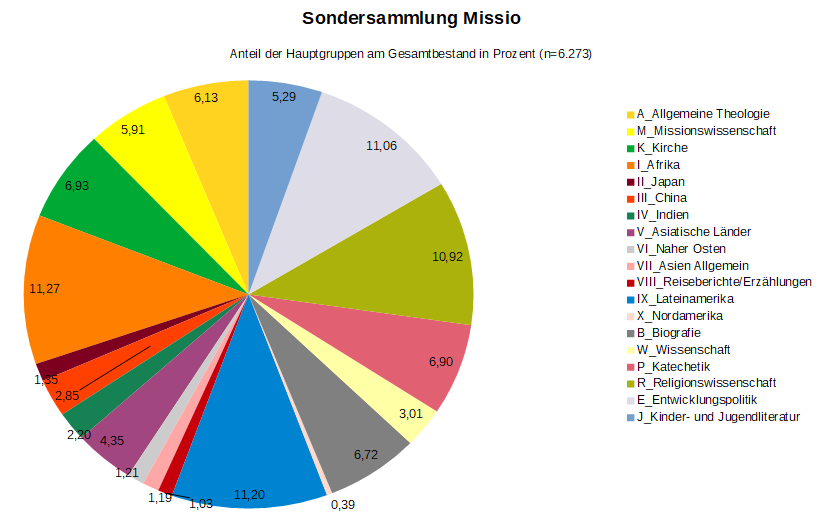
\includegraphics[width=.95\textwidth]{img/img2.PNG}
\caption{Sondersammlung Missio -- Anteil der Hauptgruppen am
Gesamtbestand in Prozent (Sparber, 2020)}
\end{figure}

Bei der Analyse der Bücher werden sowohl bildliche Darstellungen als
auch schriftliche Inhalte kolonialer Denkweisen berücksichtigt. Da keine
vollständige Textanalyse durchgeführt werden kann, werden in erster
Linie Titel, Inhaltsverzeichnisse und Einleitungen zur Beurteilung
herangezogen. Klappentexte werden nicht berücksichtigt. In jenen Fällen,
wo eine Analyse des Titels nicht möglich ist (etwa bei fehlenden
Fremdsprachenkenntnissen der Autorin), wird dieser zurückgestellt und
der nächstfolgende im Regal herangezogen.\footnote{Dies betraf Bücher in
  spanischer Sprache, die von der Autorin nicht gelesen werden konnten.}
Ein Werk wird als positiv vermerkt, sobald an einer Stelle Othering als
abwertendes Wesensmerkmal einer Einzelperson oder Gruppe erkannt wird.

Aus der Analyse lassen sich folgende Erkenntnisse ableiten:\footnote{Die
  Autorin verzichtet darauf, durch entsprechende Zitate die abwertenden
  Textstellen aus den Stichproben zu wiederholen. Um die Überprüfbarkeit
  zu gewährleisten, werden die Quellen entsprechend zitiert und im
  Quellenverzeichnis nachgewiesen.}

a) Wie aufgrund der Problemlage in der Klassifikation angenommen, sind
es vor allem Bücher in den geografischen Gruppen, in denen Othering
nachgewiesen werden konnte. Insbesondere die Hauptgruppen \emph{Afrika},
wo 41\,\% der Stichproben positiv auf soziale Abwertung befunden wurden,
\emph{Naher Osten} mit 50\,\% und \emph{Lateinamerika} mit 100\,\%
weisen entsprechende Häufungen auf. Auch wenn die Zuschreibungen an
einzelne Gruppen nicht systematisch ausgewertet wurden, sind hier
durchaus Unterschiede auszumachen. Während die indigene Bevölkerung
Südamerikas in den Büchern der Stichprobe mehrheitlich mit
paternalistischer Überheblichkeit belächelt wird,\footnote{Vergleiche
  etwa Uhlig, 1964, S. 46. Missio-Sign. IX-7/27} wird Personen aus
Afrika aber auch aus Nordamerika das Menschsein teilweise abgesprochen,
wenn sie als unzivilisiert und wild beschrieben werden.\footnote{Vergleiche
  Dodge, 1884, S. 54. Missio-Sign. IX-3/12. Das Buch, das von einer
  indigenen Bevölkerungsgruppe Nordamerikas handelt, ist wohl irrtümlich
  der Hauptgruppe Lateinamerika zugeordnet. Eventuell ist dies dem
  Begriff Indianer im Titel des Werks geschuldet.}

\begin{figure}
\centering
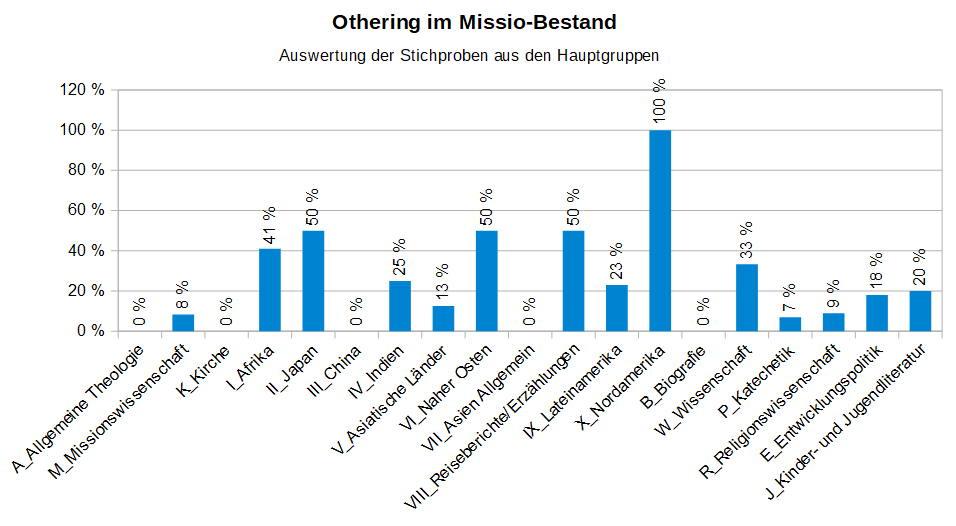
\includegraphics[width=.95\textwidth]{img/img3.png}
\caption{Othering im Missio-Bestand (Sparber, 2021)}
\end{figure}

b) In der Sondersammlung Missio sind durchaus auch zahlreiche Bücher mit
progressiven Inhalten zu finden. Auch solche Werke, die linke und
liberale Haltungen vertreten, weisen zum Teil Formen von Othering auf.
Zwei solcher Titel sind als Stichproben aus den Hauptgruppen
\emph{Nordamerika} beziehungsweise \emph{Lateinamerika} gezogen worden.
Obwohl in beiden Büchern ein Ende der Diskriminierung von Schwarzen
gefordert wird, hatte dies offensichtlich keinen Einfluss auf die
Sprachverwendung der jeweiligen Autoren.\footnote{Vergleiche Fernandes,
  1977. Missio-Sign. IX-5/80-2 und Gundolf, 1968. Missio-Sign. X-7}

c) Das zentrale Moment von Othering in den geografischen Kategorien, die
dem süd- und südöstlichen Asien zuzuordnen sind, besteht in der
Herstellung der Dichotomie christlicher und nicht-christlicher Menschen.
Obwohl die Kulturen Ost- und Südostasiens vorwiegend als hochentwickelt
beschrieben werden, entziehen sie sich einem vermeintlich europäischen
Verständnis, wenn sie beispielsweise als geheimnisvoll bezeichnet
werden.\footnote{Vergleiche Bert, 1985. Missio-Sign. IV-2/61} Des
Weiteren lässt sich bei Büchern über asiatische Länder unter
kommunistischer Führung ein ausgeprägter Antikommunismus beobachten,
weshalb nicht auszuschließen ist, dass rassistische Elemente in diesen
Fällen oft von antikommunistischen zumindest teilweise überlagert
werden. Die Stichproben ergaben stark paternalistische Perspektiven auf
das vermeintlich Fremde, das es in doppelter Hinsicht zu retten galt,
nämlich einerseits vor dem Kommunismus und andererseits vor dem falschen
Glauben. Wie für das gesamte Verhältnis zwischen Missionaren
beziehungsweise Missionarinnen und zu missionierendem Subjekt wurde
entschieden, dass Paternalismus ohne zusätzliche explizite soziale
Abwertung nicht als Form von Othering gewertet wird. Das Phänomen konnte
dadurch in keinem einzigen Buch der Stichprobe der Hauptgruppe
\emph{China} nachgewiesen werden. Auffallend im Bereich der asiatischen
Länder ist die Kategorie \emph{Japan}, wo die Hälfte der überprüften
Werke positiv zu bewerten war. Zurückzuführen ist dies auf Inhalte, in
denen Japaner als Volk mit einem tief verwurzelten Hass auf Christen
dargestellt werden, wie etwa in dem Buch mit dem vielsagenden Titel
\emph{Kreuze über Nagasaki}.\footnote{Vergleiche Huber, 1954, S. 85.
  Missio-Sign. II-1/44}

d) Jenseits der geografischen Kategorien fällt die Hauptgruppe
\emph{Wissenschaft} mit 33\,\% problematischen Inhalten in der
Stichprobe auf. In ihr finden sich rassistische Theorien in
verschiedenen Ausprägungen wie etwa im Werk des nationalsozialistischen
Ethnologen Hermann Baumann\footnote{Vergleiche Baumann, 1936, S. 6.
  Missio-Sign. R-9/15} oder den kolonialen Verlustängsten des ehemaligen
portugiesischen Ministers für die Überseegebiete, Adriano
Moreira.\footnote{Vergleiche Moreira, 1963, S. 20. Missio-Sign. E-5/10}

\hypertarget{missio-reloaded}{%
\section{Missio reloaded}\label{missio-reloaded}}

Der Frage, wo sich Othering in die Wissensorganisation der
Sondersammlung Missio eingeschrieben hat, sollte mithilfe der
historischen Bestandsanalyse nachgegangen werden. Sie wurde für die
vorliegende Arbeit designt und beruht auf der Annahme, dass sich soziale
Abwertungen als Geisteshaltung durch unsere Praktiken vermittelt in
Bibliotheksbestände einschreiben. Demnach würden wir sie in historisch
vorbelasteten wissenschaftlichen Disziplinen und somit auch in unseren,
über Klassifikationen organisierten, thematischen Schwerpunkten finden,
wo sie sich in einzelnen Werken manifestiert haben.

Tatsächlich konnten mittels Stichproben auch jene Bereiche identifiziert
werden, die eine hohe Anzahl an problematischen Inhalten aufweisen. Es
überrascht auch nicht, dass in jenen Sammelgebieten der
Missio-Bibliothek, die sich nicht direkt mit Menschen, sondern mit
religiösen Theorien, Lehren, oder Didaktik beschäftigen und die in den
Hauptgruppen \emph{Allgemeine Theologie}, \emph{Kirche} und
\emph{Katechetik} vertreten sind, kaum rassistische Inhalte vorzufinden
sind, während die praktischen Einsatzorte der Mission, in der
Klassifikation abgebildet als Regionen, Länder und Kontinente, die
höchste Anzahl an Medien beinhalten, in denen Othering betrieben wird.
Auch die drei wissenschaftlichen Hauptgruppen
\emph{Religionswissenschaft}, \emph{Wissenschaft} und
\emph{Missionswissenschaft} weisen mit durchschnittlich mehr als 15\,\%
einen nicht unwesentlichen Anteil solcher Inhalte auf.

In der praktischen Umsetzung stieß die Methode jedoch bei erzählenden
Inhalten an ihre Grenzen. Othering taucht hier meist im Kontext des
Handlungsverlaufs auf und ist in einem Schnellverfahren kaum
feststellbar. So konnte die Hauptgruppe \emph{Biografie} überhaupt nicht
ausgewertet werden. In der \emph{Kinder- und Jugendliteratur} wurden bei
20\,\% der Stichproben Dimensionen von sozialer Abwertung festgestellt.
Bei gründlicher Analyse könnte die Zahl hier jedoch höher sein.

Auf eine weitere Schwierigkeit wurde bereits hingewiesen, nämlich, dass
der Missionsgedanke selbst soziale Zuschreibungen konstruiert, die sich
in den Kategorien Gläubige und Nicht- oder Andersgläubige abbilden.
Während der Analyse war es notwendig, diese Unterscheidungen weitgehend
unberücksichtigt zu lassen, um zuverlässige Ergebnisse zu erzielen.
Festgehalten wird auch, dass der Gesamtbestand zwar viele problematische
Inhalte aufweist, gleichzeitig aber auch eine Vielzahl an Werken
beinhaltet, in denen rassistischen Ideologien vehement widersprochen
wird.

Ziel war es, mit der Analyse eine Methode zu entwickeln, mit der in
einem vereinfachten Verfahren rassistische Abwertungen in
problematischen Beständen aufzudecken sind. Auch wenn diese historische
Bestandsanalyse den angeführten Grenzen unterworfen ist, so dürfte sie
sich als Instrument zur Untersuchung kleinerer und mittlerer
Bibliotheksbestände, insbesondere solchen mit eigener Klassifikation,
eignen. Als Vorgehensweise empfehle ich ein dreistufiges Verfahren:

\begin{enumerate}
\def\labelenumi{\arabic{enumi}.}
\item
  Wissenschaftliche Kontextualisierung der inhaltlichen Schwerpunkte der
  Sammlung, um belastete Fachgebiete auszumachen.
\item
  Analyse der Klassifikation, um jene Gruppen aufzudecken, wo bereits in
  der Wissensordnung Othering nachgewiesen werden kann.
\item
  Schnellanalyse sämtlicher Schriften jener inhaltlichen Gruppen, die
  aufgrund der vorangegangenen Arbeitsschritte als anfällig für
  entsprechende Inhalte gelten sowie entsprechend adaptierte Analyse der
  Abteilungen beziehungsweise Medien mit erzählenden Inhalten.
\end{enumerate}

Im Anschluss an die Bestandsanalyse wurden die Ergebnisse dem Team der
Bibliothek der \emph{ÖFSE} präsentiert und mögliche Szenarien, wie mit
den kolonialen Repräsentationen der Sondersammlung umgegangen werden
könnte, entworfen. Da die Sondersammlung Missio innerhalb der
\emph{ÖFSE} weder als bedeutende historische missionswissenschaftliche
Bibliothek fungiert noch das Sammelgebiet der besitzenden Einrichtung
repräsentiert oder einen entsprechenden Schwerpunkt des Sammelprofils
darstellt, wurde die Empfehlung ausgesprochen, die Bücher in den
problematischen Abteilungen wie beschrieben zu analysieren und jene
Medien mit sozial abwertenden Inhalten zu entfernen.\footnote{Die Bücher
  zu entfernen soll dabei nicht als Aufforderung verstanden werden, sie
  zu entsorgen, wenngleich die Autorin diese Möglichkeit nicht
  kategorisch ausschließen möchte (etwa wenn die Bücher als historische
  Quellen an anderen Einrichtungen mit entsprechendem Sammelprofil
  ohnehin zur Verfügung stehen).} Durch eine Neuaufstellung könnte auch
auf die bestehende Klassifikation verzichtet werden. Dies würde zwar
einen nicht unwesentlichen Arbeitsaufwand darstellen, der aber als
überschaubares Projekt durchführbar wäre.

Und weiter? Wollen wir Bibliotheken als Einrichtungen verstanden wissen,
in denen wir Abwertungen von sozialen Gruppen nicht durch unsere
Praktiken reproduzieren, müssen wir uns kritisch mit bestehenden
Routinen auseinandersetzen. Auch wenn die Regale der Bibliotheken in den
wenigsten Fällen mit kolonialem Raubgut gefüllt sind, könnte etwa die
Berücksichtigung von Diskussionen innerhalb der Museumswissenschaft zu
kolonialen Kontexten unseren Blick darauf schärfen, welche Bilder von
Gruppen oder Gesellschaften wir auf den verschiedenen Ebenen
bibliothekarischen Handelns entwerfen, übernehmen beziehungsweise
vermitteln. Bibliotheken in ihrer Gesamtheit benötigen neue
Perspektiven, um als Einrichtung dem Gegenüber in seiner:ihrer
historischen, kulturellen und sozialen Verortung gerecht zu werden. Dazu
braucht es eine Vielfalt an Stimmen in einer offenen Debatte. Um
eurozentristische Paradigmen zu überwinden, wird es nicht ausreichen,
sich in der Kritik auf Ordnungssysteme und Inhalte zu beschränken.
Gleichzeitig werden Wissensordnungen weiterhin die geistigen Schablonen
darstellen, auf denen wir Gedanken formulieren, Strukturen aufbauen und
Bestände sortieren. Sie sind die \emph{episteme}, die Bedingtheit von
Wissen. Let's decolonize it!

\hypertarget{literaturverzeichnis}{%
\section{Literaturverzeichnis}\label{literaturverzeichnis}}

Il movimento attuale missionario. nelle varie nazioni (1954). Romae:
Apud Aedes Pontificiae Universitatis Gregorianae (Studia Missionalia,
8).

Bettray, Johannes (1954): Übersicht über den Stand des oesterreichischen
Missionswerkes. In: Il movimento attuale missionario. nelle varie
nazioni, Bd.~8. Romae: Apud Aedes Pontificiae Universitatis Gregorianae
(Studia Missionalia, 8), {[}31{]}--64.

Brandstetter, Anna-Maria; Hierholzer, Vera (Hg.) (2018): Nicht nur
Raubkunst! Sensible Dinge in Museen und universitären Sammlungen.
Göttingen: V\&R Unipress.

Faschingeder, Gerald (2002): Missionsgeschichte als
Beziehungsgeschichte. Die Genese des europäischen Missionseinfers als
Gegenstand der historischen Anthropologie. In: \emph{Historische
Anthropologie} 10 (1), {[}1{]}--30.

Foucault, Michel (1981): Archäologie des Wissens. Frankfurt am Main:
Suhrkamp.

Foucault, Michel (2012): Die Ordnung des Diskurses. 12. Auf. Frankfurt
am Main: Fischer Taschenbuch Verlag.

Foucault, Michel (2019): Die Ordnung der Dinge. eine Archäologie der
Humanwissenschaften. 25. Aufl. Frankfurt am Main: Suhrkamp.

Fundraising Verband Austria (Hg.) (2018): Spendenbericht 2018. Alles zum
Spendenverhalten und Spendenaufkommen in Österreich auf einen Blick.
Wien. Online verfügbar unter  \url{https://www.fundraising.at/wp-content/uploads/2019/12/Spendenbericht\_2018\_WEB.pdf}, zuletzt \linebreak geprüft am 18.05.2021.

Habermas, Rebekka (2010): Wissenstransfer und Mission. Sklavenhändler,
Missionare und Religionswissenschaftler. In: \emph{Geschichte und
Gesellschaft} 36, {[}257{]}--284. DOI:
\url{https://doi.org/10.13109/gege.2010.36.2.257}.

Kainberger, Maria (2014): Die Entstehung des "Werks der
Glaubensverbreitung" in Österreich im Lichte der Theorie vom
"Urcharisma" nach Libero Gerosa. Master-Thesis. Universität Wien, Wien.
Institut für Rechtsphilosophie.

Olson, Hope A. (2001): Sameness and difference. A cultural foundation of
classification. In: \emph{Library Ressource and Technical Services} 45
(3), S. 115--122.

Richter, Thomas (2019): Der Bestand von missio Wien in der
Missionsbibliothek und katholischen Dokumentationsstelle von missio
Aachen (MIKADO). Aachen: Institut für katholische Theologie (Aachener
Bibliothekskataloge, 1).

Schrenk, Friedemann; Kuper, Anke; Rahn, Anne Marie; Eiser, Isabel
(2018): Menschen in Sammlungen. Geschichte verpflichtet. In: Anna-Maria
Brandstetter und Vera Hierholzer (Hg.): Nicht nur Raubkunst! Sensible
Dinge in Museen und universitären Sammlungen. Göttingen: V\&R Unipress,
{[}46{]}--61, DOI: \url{https://doi.org/10.14220/9783737008082.45}.

Spivak, Gayatri Chakravorty (1985): The Rani of Sirmur. An essay in
reading the archives. In: \emph{History and theory} 24 (3), S. 247--272.
DOI: \url{https://doi.org/10.2307/2505169}.

\hypertarget{zitierte-quellen}{%
\section{Zitierte Quellen}\label{zitierte-quellen}}

Baumann, Hermann (1936): Schöpfung und Urzeit des Menschen im Mythus der
afrikanischen Völker. Berlin: Reimer.

Berg, Hans Walter (1985): Indien: Traum und Wirklichkeit. 1. Aufl.
Hamburg: Hoffmann u. Campe.

Die Integration des Negers in die Klassengesellschaft: An der Schwelle
einer neuen Zeit (1977) (5).

Dodge, Richard Irving; Mylius, Otfrid (1884): Die heutigen Indianer des
fernen Westens: Aus dreißigjähriger persönlicher Anschauung geschildert.
Wien {[}u. a.{]}: A. Hartleben.

Gundolf, Hubert (1968): Eines Tages werden wir siegen: von der Sklaverei
zum Bürgerrecht. Graz, Wien {[}u.a.{]}: Verl. Styria.

Huber, Gerhard (1954): Kreuze über Nagasaki: den sechsundzwanzig
Erstlingsmartyrern Japans zum Gedächtnis. Werl/Westf:
Dietrich-Coelde-Verl.

Moreira, Adriano (1963): Portugals Überseepolitik: Reden, Essays,
Vorträge zur gegenwärtigen Politik und Geschichte Portugals in seinen
Überseegebieten. Baden-Baden: Lutzeyer.

Uhlig, Ralf-Dieter (1964): Peru: mit Stadtführer Lima und Cuzco.
Buchenhain vor München: Mai's Reiseführer-Verl. (6).

%autor
\begin{center}\rule{0.5\linewidth}{0.5pt}\end{center}

\textbf{Sandra Sparber} leitet die Bibliothek der Psychoanalyse im
Sigmund Freud Museum Wien.

\end{document}
